
%|  Name  | TODO | ONGOING | DONE |
%|--------|------|---------|------|
%| Dana   | x    |         |      |
%| Gerd   |      |         |  x   |
%| Glenn  |      |         |  x   |
%| Jordan | x    |         |      |
%| Luke   | x    |         |      |
%| Matt   | x    |         |      |
%| Neil   | x    |         |      |
%| Scot   | x    |         |      |

In the section `IV.B. Disk Format: Level 2B - Data Object Data Storage', the HDF5 file format specification states the following regarding the storage of array values (from datasets or attributes):

\begin{quote}
Multi-dimensional array data is stored in C order; in other words, the ``last" dimension changes fastest.

Data whose elements are composed of atomic datatypes are stored in IEEE format unless they are defined explicitly as being stored in a different machine format with the architecture-type information from the datatype header message. This means that each architecture will need to [potentially] byte-swap data values into the internal representation for that particular machine.

Data with a variable-length datatype is stored in the global heap of the HDF5 file. Global heap identifiers are stored in the data object storage.

Data whose elements are composed of reference datatypes are stored in several different ways depending on the particular reference type involved. Object pointers are just stored as the offset of the object header being pointed to, with the size of the pointer being the same number of bytes as offsets in the file.

Dataset region references are stored as a heap ID, which points to the following information within the file heap: an offset of the object pointed to, number-type information (same format as header message), dimensionality information (same format as header message), sub-set start and end information (in other words, a coordinate location for each), and field start and end names (in other words, a [pointer to the] string indicating the first field included and a [pointer to the] string name for the last field).

Data of a compound datatype is stored as a contiguous stream of the items in the structure, with each item formatted according to its datatype.
\end{quote}

Having read through pages and pages of HDF5 file format intricacies, many readers may find this statement near the end of the document~\cite{ffmt} to sound anticlimactic. Undoubtedly, the writer of these lines must have run out of time or money, and he or she tried to cut corners because this sounds too simple to be true! Well, it is accurate, and the answer to the question, ``What is the HDF5 library doing to my data?" is ``Not much." or ``Not what you might be thinking." Borrowing networking terminology, the HDF5 library is \textit{framing} user data rather than manipulating the data itself. (Here, we ignore specific use cases such as datatype conversion or compression.) Similar to TCP/IP protocol layers (see Figure~\ref{fig:tcpip-protocols}), there are multiple framing layers in the HDF5 file format.

\begin{figure}[h]
    \centering
    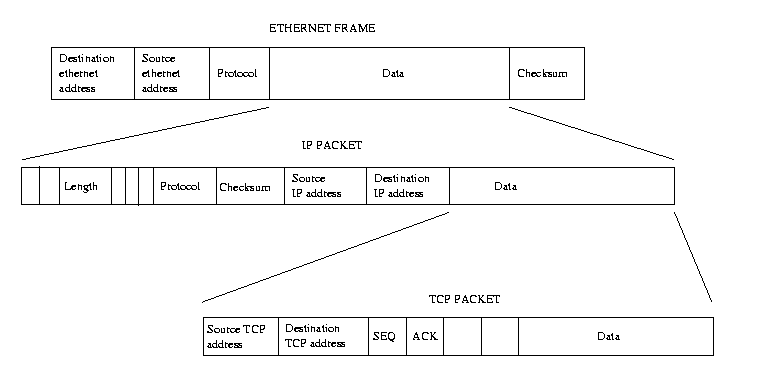
\includegraphics[width=0.75\textwidth]{images/protocols.png}
    \caption{TCP/IP Protocol Layers\cite{tldp2023}}
    \label{fig:tcpip-protocols}
\end{figure}

In this section, we explore how the native VOL performs this ``framing" of user (meta)data. After clarifying the difference between user metadata and user data, we will see why and how it treats them separately. At the end of this tour, the reader should be able to explain Figure~\ref{fig:io-paths} to their colleagues!

\subsection{User metadata and data}

Most applications using HDF5 are there to solve a scientific, engineering, or business problem. Users of the application think in terms of the particular application domain, such as particle velocities, sensor readings, or stock prices. Be that as it may, the application's creator has adopted a convention or profile on representing these domain objects using HDF5 data model entities. Like a mathematical model, in the broadest sense, the HDF5 data model is about variables and the relationships between variables. These variables, or datasets, are array variables (their values are multidimensional arrays), and relationships are expressed by arranging them in graph-like structures with labeled edges or links. Furthermore, datasets and arrangements, or groups, can be decorated by ``small'' (in the domain sense) named array variables, so-called attributes. With the ``grammar" of how these arrangements, or (logical) files, can be put together, this is essentially all there is to the HDF5 data model. In this context, we refer to dataset values (arrays!) as \textit{user data}, and everything else is considered \textit{user metadata}. In other words, user data is the ``heavy-weight" or problem-scale data, proportional to the number of degrees of freedom, the resolution, the spatio-temporal extent, etc. On the other hand, user metadata describes user data, e.g., the unit of the underlying variable, the calibration or sampling rate of an instrument, the time step, etc. Note that dataset metadata, such as rank, extent, element type, etc., is also metadata.

\begin{listing}
\centering
\caption{Dataset life cycle.}
\label{lst:dataset-life-cycle}
\begin{minted}[linenos]{C}
#include "common.h"
int main() {
    hid_t file_id = H5Fcreate("data.h5", H5F_ACC_TRUNC, H5P_DEFAULTx2);
    hid_t fspace = H5Screate_simple(1, (hsize_t[]){10}, NULL);
    hid_t dset = H5Dcreate(file_id, "data", H5T_NATIVE_INT, fspace,
        H5P_DEFAULTx3);
    H5Dclose(dset);
    H5Sclose(fspace);
    H5Fclose(file_id);
    return 0;
}
\end{minted}
\end{listing}

For example, the HDF5 data model instance created by the program in Listing~\ref{lst:dataset-life-cycle} would consist of the array \texttt{[0,0,0,0,0,0,0,0,0,0]} as its user data and metadata such as
\begin{itemize}
    \item The HDF5 file contains a single array variable linked as \texttt{data} in the root group.
    \item The element type of the array variable is ``integers between -2,147,483,648 and 2,147,483,647."
    \item The rank of the array variable is one, and its extent is ten elements.
\end{itemize}
The HDF5 library lets us persist this information in a file system's physical file \texttt{data.h5}.
In Figure~\ref{fig:io-paths}, we show the major library components involved in the framing of this information and suggest that user metadata and data are treated differently.

Following the Callgrind profile of Listing~\ref{lst:dataset-life-cycle}, a call sequence for \func{H5Dcreate} similar to the one shown in Figure~\ref{fig:tour-3-uml-dset-create-contig} emerges. Notice that we have skipped the VOL layer incantation, which applies to \func{H5Dcreate}, and we have suppressed a few details about object header composition and metadata cache entry pinning, etc. The gist of the call sequence is this:

\begin{enumerate}
    \item As a ``side-effect" of linking the newly minted dataset to the root group, we create a dataset object header conforming to the file format specification~\cite{ffmt}.
    \item The object header is placed into the file's metadata cache, and the corresponding entry is marked as dirty. That way, it will get flushed/written to the file when the metadata cache is destroyed (\func{H5AC_dest}), which happens in the wake of \func{H5Fclose}.
    \item Finally, the freshly minted dataset's file address and link name are added to the root group's symbol table, and the B-tree index is updated.
\end{enumerate}

This sequence covers the left portion of Figure~\ref{fig:io-paths}. What happened to the array? If you follow the Callgrind profile closely, you will notice that no array ever gets created and written. For one, there is no statically or dynamically allocated array in Listing~\ref{lst:dataset-life-cycle}. However, the actual reason is the default behavior of the library that prescribes so-called late allocation for datasets with contiguous layouts. Space allocation in the file is delayed until an element of the dataset is modified, which triggers the allocation and initialization with fill values for elements that aren't modified. In other words, nothing happens in the right portion of Figure~\ref{fig:io-paths} for this simple example. It's a pure metadata affair.

\begin{comment}
http://www.plantuml.com/plantuml/
@startuml
participant "H5D top" as t_h5d
participant "H5D bot." as b_h5d
participant H5L
participant H5G
participant H5O
participant H5AC
participant H5B

t_h5d -> b_h5d: H5D__create_named
b_h5d -> H5L: H5L_link_object
H5L -> H5G: H5G_traverse
H5G -> H5O: H5O_obj_create
H5O -> b_h5d: H5D__create
b_h5d -> H5O: H5O_create
rnote over H5O: H5O_create_ohdr
rnote over H5O: H5O_apply_ohdr
H5O -> H5AC: H5AC_insert_entry
H5O -> H5AC: H5AC_mark_entry_entry
H5L -> H5G: H5G_obj_insert
H5G -> H5O: H5O_link
rnote over H5G: H5G_stab_insert
H5G -> H5B: H5B_insert
H5B -> H5G: H5G__node_insert
@enduml
\end{comment}

\begin{figure}
    \centering
    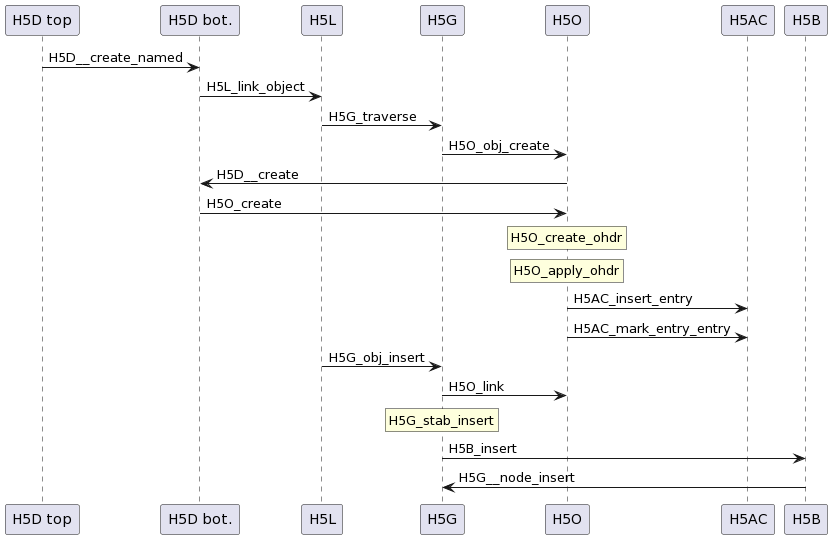
\includegraphics[width=0.80\textwidth]{images/tour_3_uml_dset_create.png}
    \caption{Process to create a contiguous dataset.}
    \label{fig:tour-3-uml-dset-create-contig}
\end{figure}

The dataflow for datasets is similar to files in that the in-memory representation has top (\texttt{H5D\_t}) and bottom (\texttt{H5D\_shared\_t}) portions. Both are defined in \texttt{H5Dpkg.h}. The top portion is unique to each instance of an opened dataset, and the bottom portion is a shared struct that is only created once for a given dataset. (The dataset's object header is constructed from the information in the bottom portion.) Thus, if a dataset is opened twice, there will be two handles (IDs) and two \texttt{H5D\_t} structs, both sharing one \texttt{H5D\_shared\_t}.

\subsection{Data transfer}\label{sec:data-transfer}

To activate the right portion of Figure~\ref{fig:io-paths}, we call \func{H5Dwrite}, as shown in Listing~\ref{lst:dataset-transfer}. The key elements of the user data journey are captured in Figure~\ref{fig:tour-3-uml-dset-write-contig}. We can see that storage for the data is allocated in the file. There is, however, a twist: the data is not written into the file when \func{H5Dwrite} is called or completed. Because the array to be written is so small, the data is copied to a buffer, and the write is delayed until the dataset is closed, when it is flushed (\func{H5D__flush_sieve_buf}). The native VOL uses a so-called data sieve buffer to reduce the number of small I/O operations. (We will have more to say about the sieve buffer in section~\ref{sec:tour6}.)

\begin{listing}
\centering
\caption{Data transfer.}
\label{lst:dataset-transfer}
\begin{minted}[linenos]{C}
#include "common.h"
int main() {
    hid_t file_id = H5Fcreate("data.1.h5", H5F_ACC_TRUNC, H5P_DEFAULTx2);
    hid_t fspace = H5Screate_simple(1, (hsize_t[]){10}, NULL);
    hid_t dset = H5Dcreate(file_id, "data", H5T_NATIVE_INT, fspace,
        H5P_DEFAULTx3);
    int data[10] = {0,1,2,3,4,5,6,7,8,9};
    H5Dwrite(dset, H5T_NATIVE_INT, H5S_ALL, H5S_ALL, H5P_DEFAULT, data);
    H5Dclose(dset);
    H5Sclose(fspace);
    H5Fclose(file_id);
    return 0;
}
\end{minted}
\end{listing}

\begin{comment}
http://www.plantuml.com/plantuml/
@startuml
participant "H5D top" as t_h5d
participant "H5D bot." as b_h5d
participant H5FL
participant H5FD

t_h5d -> b_h5d: H5VL__native_dataset_write
rnote over b_h5d: H5D__write
rnote over b_h5d: H5D__ioinfo_init
rnote over b_h5d: H5D__alloc_storage
rnote over b_h5d: H5D__contig_write
rnote over b_h5d: H5D__select_io
rnote over b_h5d: H5D__contig_writevv
rnote over b_h5d: H5D__contig_writevv_sieve_cb
b_h5d -> H5FL: H5FL_blk_calloc
t_h5d -> b_h5d: H5VL__native_dataset_close
rnote over b_h5d: H5D_close
rnote over b_h5d: H5D__contig_flush
rnote over b_h5d: H5D__flush_sieve_buf

b_h5d -> H5FD: H5FD_write
rnote over H5FD: H5FD__sec2_write
@enduml
\end{comment}

\begin{figure}
    \centering
    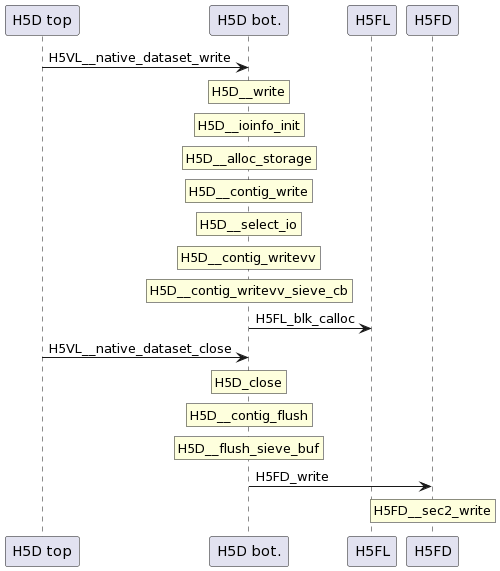
\includegraphics[width=0.55\textwidth]{images/tour_3_uml_dset_write.png}
    \caption{Process to write a (small) contiguous dataset.}
    \label{fig:tour-3-uml-dset-write-contig}
\end{figure}


\subsection{Chunked storage layouts, selections \& partial I/O}\label{sec:layouts-selections}

The flow discussed in section~\ref{sec:data-transfer} places us in the right portion of Figure~\ref{fig:io-paths}. However, we haven't exercised much of the machinery shown there. To activate a few of those components, we modify the storage layout and write only parts of the dataset, as shown in Listing~\ref{lst:dataset-chunky}.

\begin{listing}
\centering
\caption{Data -- chunked layout, selection, \& partial I/O.}
\label{lst:dataset-chunky}
\begin{minted}[linenos]{C}
#include "common.h"
int main() {
    hid_t file = H5Fcreate("data.3.1.h5", H5F_ACC_TRUNC, H5P_DEFAULTx2);
    hid_t fspace = H5Screate_simple(1, (hsize_t[]){10}, NULL);
    hid_t dcpl = H5Pcreate(H5P_DATASET_CREATE);
    H5Pset_chunk(dcpl, 1, (hsize_t[]){6});
    hid_t dset = H5Dcreate(file, "data", H5T_NATIVE_INT, fspace,
        H5P_DEFAULT, dcpl, H5P_DEFAULT);
    int data[5] = {1,3,5,7,9};
    hid_t mspace = H5Screate_simple(1, (hsize_t[]){5}, NULL);
    H5Sselect_all(mspace);
    H5Sselect_hyperslab(fspace, H5S_SELECT_SET, (hsize_t[]){1}, (hsize_t[]){2},
        (hsize_t[]){5}, (hsize_t[]){1});
    H5Dwrite(dset, H5T_NATIVE_INT, mspace, fspace, H5P_DEFAULT, data);
    H5Dclose(dset);
    H5Sclose(mspace);
    H5Pclose(dcpl);
    H5Sclose(fspace);
    H5Fclose(file);
    return 0;
}
\end{minted}
\end{listing}

The changes compared to the sequence shown in Figure~\ref{fig:tour-3-uml-dset-write-contig} are shown in Figure~\ref{fig:tour-3-uml-dset-write-chunk}.

\begin{comment}
http://www.plantuml.com/plantuml/
@startuml
participant "H5D top" as t_h5d
participant "H5D bot." as b_h5d
participant H5B
participant H5S
participant H5F

hnote over b_h5d #FFAAAA: Change in storage allocation

rnote over b_h5d: H5D__create
rnote over b_h5d: H5D__update_oh_info
rnote over b_h5d: H5D__layout_oh_create
rnote over b_h5d: H5D__chunk_init
rnote over b_h5d: H5D__btree_idx_init
b_h5d -> H5B: H5B_shared_new

hnote over H5S #FFAAAA: Selection construction

rnote over H5S: H5S_select_hyperslab
rnote over H5S: H5S__hyper_regular_and_single_block
rnote over H5S: H5S__generate_hyper_slab
rnote over H5S: H5S__make_hyper_spans

hnote over b_h5d #FFAAAA: Change in write path

t_h5d -> b_h5d: H5VL__native_dataset_write
rnote over b_h5d: H5D__write
rnote over b_h5d: H5D__chunk_io_init
rnote over b_h5d: H5D__alloc_storage
rnote over b_h5d: H5D__chunk_create
rnote over b_h5d: H5D__chunk_write
rnote over b_h5d: H5D__select_write
rnote over b_h5d: H5D__select_iter_init

hnote over b_h5d #FFAAAA: Change in dataset close
t_h5d -> b_h5d: H5VL__native_dataset_close
rnote over b_h5d: H5D_close
rnote over b_h5d: H5D__chunk_flush
rnote over b_h5d: H5D__chunk_file_alloc
b_h5d -> H5F: H5F_shared_block_write
rnote over b_h5d: H5D__btree_idx_insert
rnote over b_h5d: H5D__chunk_cinfo_cache_update
@enduml
\end{comment}

\begin{figure}
    \centering
    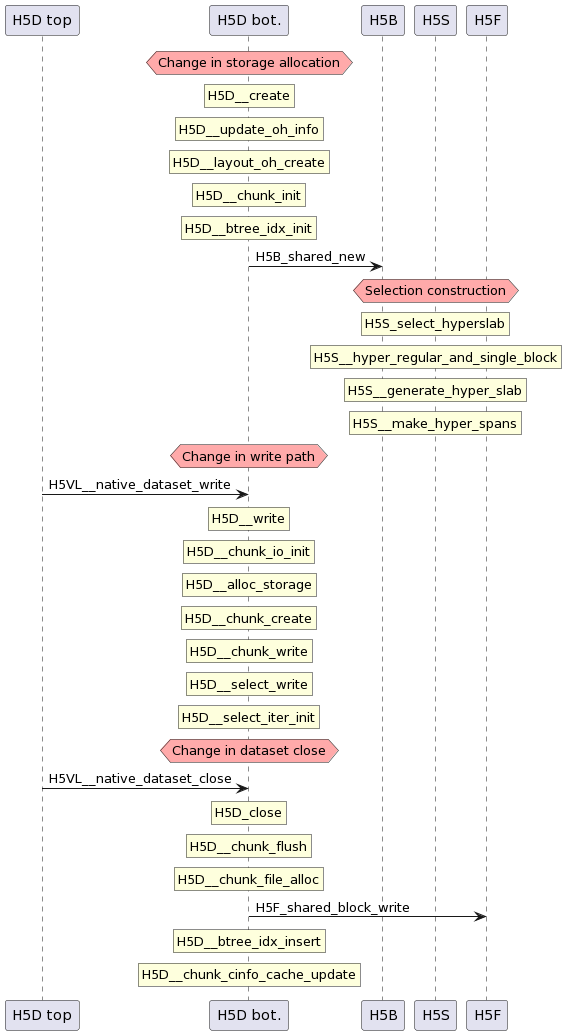
\includegraphics[width=0.55\textwidth]{images/tour_3_uml_dset_write_sel.png}
    \caption{Process to write a selection to a (small) chunked dataset.}
    \label{fig:tour-3-uml-dset-write-chunk}
\end{figure}

The gist is this:
\begin{enumerate}
    \item The different storage layout (chunked) is noted in the dataset's object header at creation time. The chunk locations are tracked with a B-tree index. Not that, as in the contiguous case, chunk allocation is delayed until any actual data is written.
    \item The hyperslab selection construction is a 100\% in-memory metadata affair and is \textit{not} routed through the VOL interface.
    \item The function \func{H5Dwrite} is responsible for allocating chunks and iterating through selections. However, data is not written immediately if the array and chunk sizes are small. Instead, it is written only after the dataset is closed and flushed. The actual writing of user data is done by \func{H5F_shared_block_write}. After writing, the chunk index is updated.
\end{enumerate}

While we have not yet explored the native VOLs facilities for datatype conversion, data filtering, or data caching and buffering, we have seen enough to corroborate the claim that the native VOL does not alter user data. Instead, it frames the data and augments them with metadata to create a self-describing package called a native HDF5 file. In section~\ref{sec:user-metadata}, we explore how an everyday kind of user-metadata, attributes, fares under the scheme outlined in Figure~\ref{fig:io-paths}.

\subsection{User-defined metadata -- The life cycle of an HDF5 attribute}\label{sec:user-metadata}

\paragraph{Overview} Attributes' purpose is to associate metadata with HDF5 objects directly. Attributes have a very similar interface to datasets - they have a layout defined by a dataspace, contain user data with a datatype determined at creation, and can be written to and read from. Attribute operations pass through the Virtual Object Layer to reach the active VOL connector's storage implementation.

Because attributes exist primarily as metadata, they are distinct from datasets in a few key ways. Attributes are always associated with a parent object: a dataset, group, or committed datatype. Attributes can only be accessed through their parent object, and attribute names are significant only within that parent object. Because they exist entirely as metadata in storage by default, attributes should generally contain less than 64KiB of data (see the "Attribute storage layouts" section for handling larger attributes). For the same reason, an attribute's data must be read or written entirely in every access; partial reading or writing using a selection is not allowed.

\begin{listing}
\centering
\caption{Attribute life cycle.}
\label{lst:attribute-life-cycle}
\begin{minted}[linenos]{C}
#include "common.h"
int main() {
  hid_t file_id = H5Fcreate("attrib.1.h5", H5F_ACC_TRUNC, H5P_DEFAULTx2);
  hid_t scalar = H5Screate(H5S_SCALAR);
  hid_t attr_id =
      H5Acreate(file_id, "meta", H5T_NATIVE_INT, scalar, H5P_DEFAULTx2);
  int meta = 42;
  H5Awrite(attr_id, H5T_NATIVE_INT, &meta);
  H5Aclose(attr_id);
  H5Sclose(scalar);
  H5Fclose(file_id);
  return 0;
}
\end{minted}
\end{listing}

\paragraph{Attributes as objects} Listing~\ref{lst:attribute-life-cycle} shows the life cycle of an attribute. It is created on a parent object, in this case (the root group of) the file \texttt{attrib.1.h5}. It is created with a dataspace and datatype defining the data it stores. Data is written to the attribute in storage, and then the in-memory object for the attribute is closed.

\begin{listing}
\centering
\caption{Dense storage used with many attributes}
\label{lst:attribute-dense-storage-many}
\begin{minted}[linenos]{C}
#include "common.h"
int main() {
  hid_t fapl_id = H5Pcreate(H5P_FILE_ACCESS);
  hid_t fcpl_id = H5Pcreate(H5P_FILE_CREATE);
  H5Pset_libver_bounds(fapl_id, H5F_LIBVER_V18, H5F_LIBVER_LATEST);
  /* Max in compact storage = 2, min in dense storage = 2 */
  H5Pset_attr_phase_change(fcpl_id, 2, 2);
  hid_t file_id =
    H5Fcreate("attrib.2.h5", H5F_ACC_TRUNC, H5P_DEFAULT, fapl_id);
  hid_t scalar = H5Screate(H5S_SCALAR);
  hid_t attr_id1 =
      H5Acreate(file_id, "attr1", H5T_NATIVE_INT, scalar, H5P_DEFAULTx2);
  hid_t attr_id2 =
      H5Acreate(file_id, "attr2", H5T_NATIVE_INT, scalar, H5P_DEFAULTx2);
  /* More than 2 compact attributes - all are moved to dense */
  hid_t attr_id3 =
      H5Acreate(file_id, "attr3", H5T_NATIVE_INT, scalar, H5P_DEFAULTx2);
  H5Aclose(attr_id1);
  H5Aclose(attr_id2);
  H5Aclose(attr_id3);
  H5Adelete(file_id, "attr2");
  H5Adelete(file_id, "attr3");
  /* Less than 2 dense attributes - the rest are moved to compact */
  H5Sclose(scalar);
  H5Fclose(file_id);
  H5Pclose(fapl_id);
  H5Pclose(fcpl_id);
  return 0;
}
\end{minted}
\end{listing}

When an attribute is opened, the library handle points to an instance of \texttt{H5A\_t}. The shared attribute information attached to this structure contains pointers to the attribute's datatype and dataspace, as well as its creation index on its parent object if creation index tracking was enabled at object creation time. Because the creation index is only computed when the attribute is first created or opened, operations such as removing attributes could cause it to become invalid (e.g. its creation index could exceed the total number of attributes on the parent object). This is why, before an attribute is deleted from its parent object, identifiers of other attributes on that object should be closed, and only re-opened after the attribute deletion is complete.

\begin{listing}
\centering
\caption{Dense storage used with a large attribute}
\label{lst:attribute-dense-storage-large}
\begin{minted}[linenos]{C}
#include "common.h"
int main() {
  hid_t fapl_id = H5Pcreate(H5P_FILE_ACCESS);
  H5Pset_libver_bounds(fapl_id, H5F_LIBVER_V18, H5F_LIBVER_LATEST);
  hid_t file_id =
    H5Fcreate("attrib.3.h5", H5F_ACC_TRUNC, H5P_DEFAULT, fapl_id);
  hid_t scalar = H5Screate(H5S_SCALAR);
  /* One element is 4*2*512*512 = ~4194K bytes (with 4-byte integers)
   * Will automatically be put into dense storage */
  hid_t dtype = H5Tarray_create(H5T_NATIVE_INT, 2, (hsize_t[]){512, 512});
  hid_t attr_id = H5Acreate(file_id, "image", dtype, scalar, H5P_DEFAULTx2);
  int meta[512][512];
  H5Awrite(attr_id, dtype, &meta);
  H5Aclose(attr_id);
  H5Tclose(dtype);
  H5Sclose(scalar);
  H5Fclose(file_id);
  H5Pclose(fapl_id);
  return 0;
}
\end{minted}
\end{listing}


\subsection{Attribute storage layouts}

\paragraph{Overview} There are two primary ways that attributes may be stored - 'compact' storage and 'dense' storage. Compact attributes are small and few in number, and are stored in the header of their parent object. Dense attributes are large or many in number, and are stored in the file's global fractal heap. There is a technique that could be considered a third metadata storage method: Using attributes with reference datatypes to point at metadata stored in other objects.

\paragraph{Compact Storage} When attributes are in compact storage, they are stored as attribute messages in the object header of their parent object. An attribute is stored compactly if it is below 64KiB in size and the parent object's total number of attributes is below its max compact storage threshold defined by \func{H5Pset_attr_phase_change}.

Figure~\ref{fig:tour-3-uml-attr-create-compact} is a diagram of the library's internal process to create an attribute in compact storage with the native VOL connector. First, \func{H5O__attr_create} uses \func{H5O_pin} to 'pin' the object header, preventing it from being flushed from the cache to storage until it is unpinned at the end of the operation. Once it is determined that the new attribute should be compact, \func{H5O__msg_append_real} handles creating the new attribute message and inserting it into the object header. This is done in two steps: First, \func{H5O__msg_alloc} creates a new message in the header, and returns its location within the header. Then, \func{H5O__copy_mesg} uses the copy callback of the message type to populate the newly created message. In this case, the new message is an attribute message providing the copy callback \func{H5O__attr_copy}, a wrapper around the library's function for copying attributes, \texttt{H5A\_\_copy()}. The generic attribute copy function may be used here because attribute messages contain copies of the native \texttt{H5A\_t} object.

\begin{comment}
http://www.plantuml.com/plantuml/
@startuml
participant H5A
participant H5O

H5A -> H5O: H5A__create
rnote over H5O: H5O__attr_create()

hnote over H5O #FFAAAA: Object header is pinned

rnote over H5O: H5O__msg_append_real
rnote over H5O: H5O__msg_alloc
rnote over H5O: H5O__copy_mesg
H5O -> H5A: H5O__attr_copy
rnote over H5A: H5A__copy

hnote over H5O #FFAAAA: Object header is unpinned
@enduml
\end{comment}

\begin{figure}
    \centering
    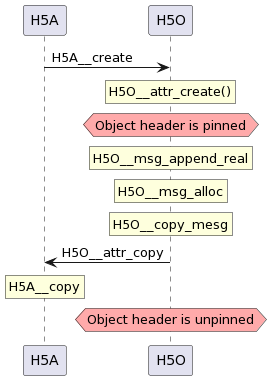
\includegraphics[width=0.30\textwidth]{images/tour_3_uml_attr_create_compact.png}
    \caption{Process to create a compact attribute}
    \label{fig:tour-3-uml-attr-create-compact}
\end{figure}

Figure~\ref{fig:tour-3-uml-attr-remove-compact} is a diagram of the library's internal process to remove a compact attribute. Once again, the object header is pinned to prevent it from being flushed during an operation. The attribute messages in the object header are iterated over in \func{H5O__mesg_iterate_real}, and the callback \func{H5O__attr_remove_cb} is executed on each. If the attribute message matches the name of the attribute to be deleted, then the deletion process is performed by \func{H5O__release_mesg}. The removal of the object header message takes place in two parts: first, \func{H5O__delete_msg} is used to invoke the attribute message's delete callback, \func{H5O__attr_delete}, which deletes header messages that were referred to by this attribute - specifically, dataspace and datatype messages. After that, \func{H5O__msg_free_mesg} invokes the attribute message's 'free' callback, to free the native information stored in the attribute message - the \texttt{H5A\_t} structure and its associated memory.

\begin{comment}
http://www.plantuml.com/plantuml/
@startuml
participant H5A
participant H5O

rnote over H5A: H5Adelete
H5A -> H5O: (...)
rnote over H5O: H5O__attr_remove

hnote over H5O #FFAAAA: Object header is pinned
rnote over H5O: H5O__msg_iterate_real
H5O -> H5O: Attr msg found
rnote over H5O: H5O__attr_remove_cb
rnote over H5O: H5O__release_mesg
rnote over H5O: H5O__delete_mesg
H5O -> H5O: H5O__attr_delete

H5O -> H5A: H5O__msg_free_mesg
rnote over H5A: H5A__close

hnote over H5O #FFAAAA: Object header is unpinned
@enduml
\end{comment}

\begin{figure}
    \centering
    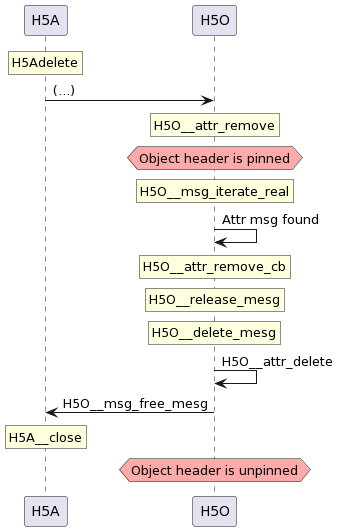
\includegraphics[width=0.35\textwidth]{images/tour_3_uml_attr_remove_compact.png}
    \caption{Removal of a compact attribute}
    \label{fig:tour-3-uml-attr-remove-compact}
\end{figure}

Compact attributes have some drawbacks - performance suffers when objects have many compact attributes and they are strictly limited in size to fit within the object header.  Both of these limitations are circumvented by dense storage.

\paragraph{Dense Storage} When an attribute is in dense storage, the object header contains a pointer to the location of the attribute's data on disk rather than containing the attribute's data directly.

\begin{comment}
http://www.plantuml.com/plantuml
@startuml
participant H5A
participant H5O
participant H5HF
participant H5B2

H5A -> H5O: H5A__create
rnote over H5O: H5O__attr_create()
hnote over H5O #FFAAAA: Object header is pinned
H5O -> H5A:

opt Fractal heap does not yet exist
rnote over H5A: H5A__dense_create
H5A -> H5HF: Create fractal heap in the file
rnote over H5HF: H5HF_create
H5A -> H5B2: Create name index B-tree
rnote over H5B2: H5B2_create

opt If ceation order is tracked
H5A -> H5B2: Create creation order B-tree
rnote over H5B2: H5B2_create
end
end

rnote over H5A: H5A__dense_insert

alt If attribute message is shared
rnote over H5A: Copy pre-existing heap ID
else Attribute message is not shared

H5A -> H5HF: Insert attr into fractal heap
rnote over H5HF: H5HF_insert
end

H5A -> H5B2: Insert attr name into name B-tree
rnote over H5B2: H5B2_insert

opt If creation order is tracked
H5A -> H5B2: Insert record into creation order B-tree
rnote over H5B2: H5B2_insert
end

hnote over H5O #FFAAAA: Object header is unpinned
@enduml
\end{comment}

\begin{figure}
    \centering
    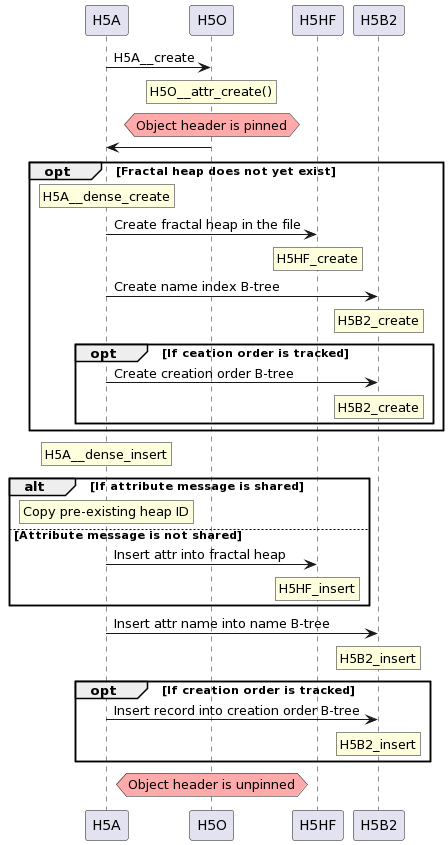
\includegraphics[width=0.5\textwidth]{images/tour_3_uml_attr_create_dense.png}
    \caption{Attribute insertion into dense storage}
    \label{fig:tour-3-uml-attr-create-dense}
\end{figure}

\begin{comment}
http://www.plantuml.com/plantuml
@startuml
participant H5A
participant H5O

rnote over H5A: H5Adelete
H5A -> H5O: (...)
rnote over H5O: H5O__attr_remove

hnote over H5O #FFAAAA: Object header is pinned
H5O -> H5A:
rnote over H5A: H5A__dense_remove
H5A -> H5B2: Remove from name index B-tree
rnote over H5B2: H5B2_remove

opt Creation order is tracked
H5A -> H5B2: Remove from creation order B-tree
rnote over H5B2: H5B2_remove
end

alt If attribute is shared
H5A -> H5SM:
rnote over H5SM: H5SM_delete

else If attribute is not shared
H5A -> H5O: Delete dtype/dataspace
rnote over H5O: H5O__attr_delete
H5A -> H5HF:
rnote over H5HF: H5HF_remove
end

hnote over H5O #FFAAAA: Object header is unpinned
@enduml
\end{comment}

\begin{figure}
    \centering
    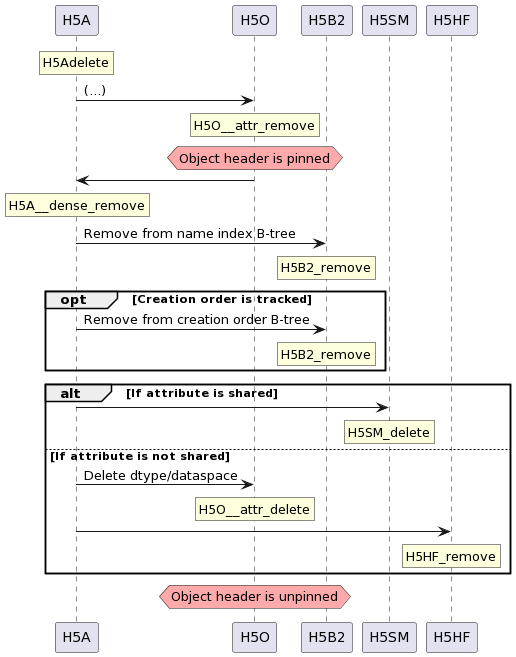
\includegraphics[width=0.65\textwidth]{images/tour_3_uml_attr_remove_dense}
    \caption{Attribute deletion in dense storage}
    \label{fig:tour-3-uml-attr-remove-dense}
\end{figure}

There are two circumstances under which a new attribute is placed into dense storage. The first is that the number of attributes on the parent object exceeds the maximum number of compact attributes on the object. This threshold may be specified for each object using \func{H5P_set_attr_phase_change}. The second is that the size of the attribute exceeds 64k bytes, and it would not fit into compact storage. All pre-existing attributes are moved to dense storage whenever a new attribute is placed into dense storage.

Figure~\ref{fig:tour-3-uml-attr-create-dense} shows the library's internal process to create an attribute in dense storage. The object header is still pinned, even though the new attribute is not to be stored in the object header. This is because the attribute creation may have side effects that require modifying the object header. If this file does not yet have a fractal heap for dense attribute storage, one is created with \func{H5A__dense_create}. This step also involves the creation of a B-tree to map dense attribute names to attribute information and optionally creating a B-tree to make the attribute information available by creation order. Once the dense attribute storage structures are confirmed, the attribute's information is stored densely by \func{H5A__dense_insert}. This involves using the attribute message's encode callback to serialize the attribute, and this serialized attribute information is inserted into the fractal heap by \func{H5HF_insert}. If the attribute is shared, then this attribute points to the information of an attribute that already exists in the fractal heap. In this case, the insertion into the fractal heap is skipped, and the heap ID of the existing attribute in the fractal heap is copied. The heap information of the new attribute (or preexisting shared attribute) is stored in the name-index B-tree, to be accessed later by the hash of the attribute name. Lastly, if the creation order is tracked, the heap information is also inserted into the creation-order B-tree, to be accessed later by link creation order.

Figure~\ref{fig:tour-3-uml-attr-remove-dense} shows the library's internal process to remove an attribute from dense storage. After \func{H5O__attr_remove} determines the target attribute is in dense storage, \func{H5A__dense_remove} performs the removal. \func{H5B2_remove} searches the name-index B-tree and removes the information for the dense link. If creation order is tracked, the same operation is performed on the creation order B-tree. If the dense attribute is shared between objects, the 'deletion' is handled by using \func{H5SM_delete} to decrease the reference count of the shared attribute message. Otherwise, the dense attribute's referenced information (dataspace/datatype messages) is deleted by \func{H5O__attr_delete}, and it is removed from the dense attribute fractal heap.

When an attribute is removed from storage, the remaining attributes may be moved back into compact storage. If two conditions are met, an attribute will be moved back to compact storage. First, the total number of remaining attributes must be below the minimum number of dense attributes on the object, another threshold set by \func{H5P_set_attr_phase_change}. Second, the attribute must be under 64k bytes in size. It is possible for the removal of an attribute to cause some, but not all, of the remaining attributes to be moved to compact storage due to some being too large to store compactly.

\paragraph{Attribute Storage and File Format Versions}  Note that because it affects how the HDF5 file is stored on disk, using dense attribute storage requires allowing the library to use a 1.8+ version of the file format (i.e. using \func{H5Pset_libver_bounds} with a low version $\geq$ 1.8). With a pre-1.8 compatible file format version, attribute storage will always be compact, and attempts to create attributes greater than 64KiB in size will fail. Pre-1.8 compatible large metadata storage can be accomplished by storing metadata as datasets.

\subsection{Summary}

Attributes provide a flexible way to store metadata on an HDF5 object with the same CRUD interface as datasets. By default, attributes are stored compactly in the object header with other object metadata. The library takes advantage of the properties of B-trees and fractal heaps for large attributes or large amounts of attributes. If backward compatibility or compressibility is required for metadata, it may be stored in datasets and accessed from other objects through references.

From the perspective of the native VOL, user metadata and data travel down two different ``swim lanes," as depicted in Figure~\ref{fig:io-paths}. The main reason is their different role and functions in the HDF5 data model, which leads to different operations being supported in efficient and practical implementations.

\begin{landscape}
\begin{sidewaysfigure}[!ht]
%\begin{figure}[h!]
\centering
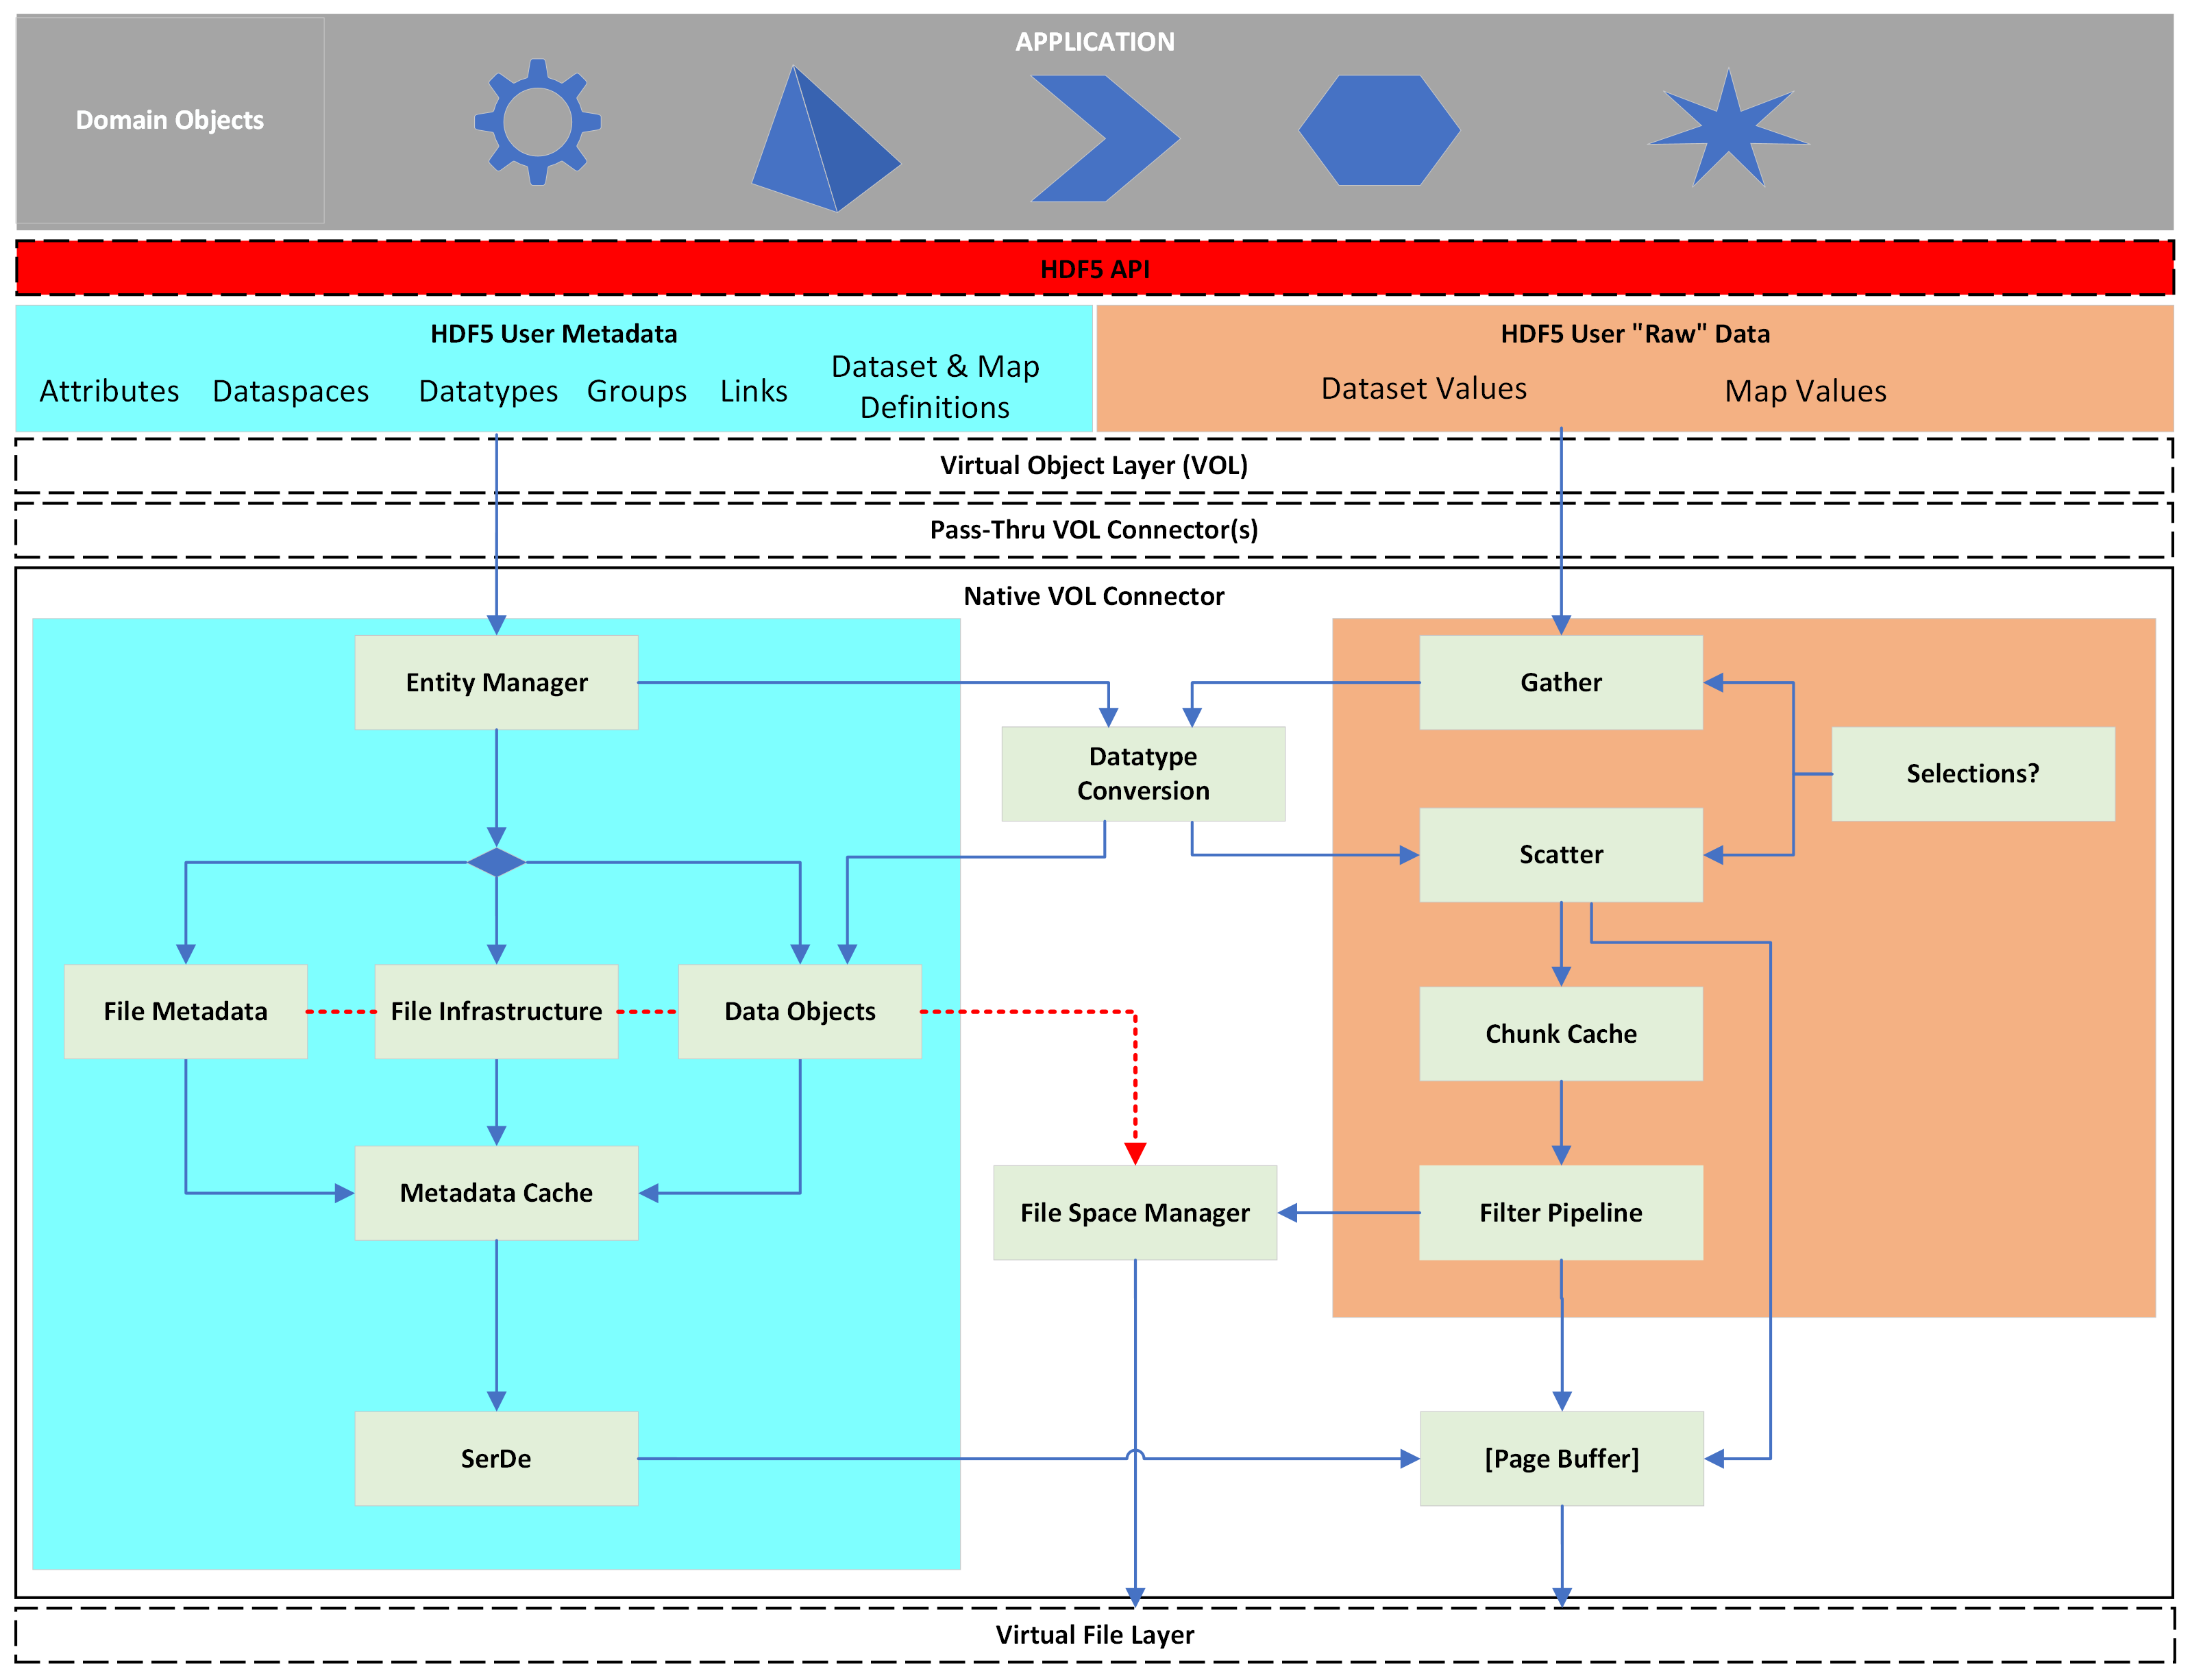
\includegraphics[scale=0.74,angle=90]{images/HDF5 library meta data.png}
\caption{The different I/O paths for metadata and ``raw'' data through the HDF5 library.\label{fig:io-paths}}
%\end{figure}
\end{sidewaysfigure}
\end{landscape}
